\documentclass[11pt,]{article}
\usepackage[left=1in,top=1in,right=1in,bottom=1in]{geometry}
\newcommand*{\authorfont}{\fontfamily{phv}\selectfont}
\usepackage[]{mathpazo}


  \usepackage[T1]{fontenc}
  \usepackage[utf8]{inputenc}




\usepackage{abstract}
\renewcommand{\abstractname}{}    % clear the title
\renewcommand{\absnamepos}{empty} % originally center

\renewenvironment{abstract}
 {{%
    \setlength{\leftmargin}{0mm}
    \setlength{\rightmargin}{\leftmargin}%
  }%
  \relax}
 {\endlist}

\makeatletter
\def\@maketitle{%
  \newpage
%  \null
%  \vskip 2em%
%  \begin{center}%
  \let \footnote \thanks
    {\fontsize{18}{20}\selectfont\raggedright  \setlength{\parindent}{0pt} \@title \par}%
}
%\fi
\makeatother




\setcounter{secnumdepth}{0}

\usepackage{color}
\usepackage{fancyvrb}
\newcommand{\VerbBar}{|}
\newcommand{\VERB}{\Verb[commandchars=\\\{\}]}
\DefineVerbatimEnvironment{Highlighting}{Verbatim}{commandchars=\\\{\}}
% Add ',fontsize=\small' for more characters per line
\usepackage{framed}
\definecolor{shadecolor}{RGB}{248,248,248}
\newenvironment{Shaded}{\begin{snugshade}}{\end{snugshade}}
\newcommand{\AlertTok}[1]{\textcolor[rgb]{0.94,0.16,0.16}{#1}}
\newcommand{\AnnotationTok}[1]{\textcolor[rgb]{0.56,0.35,0.01}{\textbf{\textit{#1}}}}
\newcommand{\AttributeTok}[1]{\textcolor[rgb]{0.77,0.63,0.00}{#1}}
\newcommand{\BaseNTok}[1]{\textcolor[rgb]{0.00,0.00,0.81}{#1}}
\newcommand{\BuiltInTok}[1]{#1}
\newcommand{\CharTok}[1]{\textcolor[rgb]{0.31,0.60,0.02}{#1}}
\newcommand{\CommentTok}[1]{\textcolor[rgb]{0.56,0.35,0.01}{\textit{#1}}}
\newcommand{\CommentVarTok}[1]{\textcolor[rgb]{0.56,0.35,0.01}{\textbf{\textit{#1}}}}
\newcommand{\ConstantTok}[1]{\textcolor[rgb]{0.00,0.00,0.00}{#1}}
\newcommand{\ControlFlowTok}[1]{\textcolor[rgb]{0.13,0.29,0.53}{\textbf{#1}}}
\newcommand{\DataTypeTok}[1]{\textcolor[rgb]{0.13,0.29,0.53}{#1}}
\newcommand{\DecValTok}[1]{\textcolor[rgb]{0.00,0.00,0.81}{#1}}
\newcommand{\DocumentationTok}[1]{\textcolor[rgb]{0.56,0.35,0.01}{\textbf{\textit{#1}}}}
\newcommand{\ErrorTok}[1]{\textcolor[rgb]{0.64,0.00,0.00}{\textbf{#1}}}
\newcommand{\ExtensionTok}[1]{#1}
\newcommand{\FloatTok}[1]{\textcolor[rgb]{0.00,0.00,0.81}{#1}}
\newcommand{\FunctionTok}[1]{\textcolor[rgb]{0.00,0.00,0.00}{#1}}
\newcommand{\ImportTok}[1]{#1}
\newcommand{\InformationTok}[1]{\textcolor[rgb]{0.56,0.35,0.01}{\textbf{\textit{#1}}}}
\newcommand{\KeywordTok}[1]{\textcolor[rgb]{0.13,0.29,0.53}{\textbf{#1}}}
\newcommand{\NormalTok}[1]{#1}
\newcommand{\OperatorTok}[1]{\textcolor[rgb]{0.81,0.36,0.00}{\textbf{#1}}}
\newcommand{\OtherTok}[1]{\textcolor[rgb]{0.56,0.35,0.01}{#1}}
\newcommand{\PreprocessorTok}[1]{\textcolor[rgb]{0.56,0.35,0.01}{\textit{#1}}}
\newcommand{\RegionMarkerTok}[1]{#1}
\newcommand{\SpecialCharTok}[1]{\textcolor[rgb]{0.00,0.00,0.00}{#1}}
\newcommand{\SpecialStringTok}[1]{\textcolor[rgb]{0.31,0.60,0.02}{#1}}
\newcommand{\StringTok}[1]{\textcolor[rgb]{0.31,0.60,0.02}{#1}}
\newcommand{\VariableTok}[1]{\textcolor[rgb]{0.00,0.00,0.00}{#1}}
\newcommand{\VerbatimStringTok}[1]{\textcolor[rgb]{0.31,0.60,0.02}{#1}}
\newcommand{\WarningTok}[1]{\textcolor[rgb]{0.56,0.35,0.01}{\textbf{\textit{#1}}}}

\usepackage{graphicx,grffile}
\makeatletter
\def\maxwidth{\ifdim\Gin@nat@width>\linewidth\linewidth\else\Gin@nat@width\fi}
\def\maxheight{\ifdim\Gin@nat@height>\textheight\textheight\else\Gin@nat@height\fi}
\makeatother
% Scale images if necessary, so that they will not overflow the page
% margins by default, and it is still possible to overwrite the defaults
% using explicit options in \includegraphics[width, height, ...]{}
\setkeys{Gin}{width=\maxwidth,height=\maxheight,keepaspectratio}


\title{Statistical Analysis of Temporal and Spatial Trends in US Covid-19 Cases
and Deaths  }



\author{\Large Jason Gong and Micah Swann\vspace{0.05in} \newline\normalsize\emph{University of California, Davis}  }


\date{}

\usepackage{titlesec}

\titleformat*{\section}{\normalsize\bfseries}
\titleformat*{\subsection}{\normalsize\itshape}
\titleformat*{\subsubsection}{\normalsize\itshape}
\titleformat*{\paragraph}{\normalsize\itshape}
\titleformat*{\subparagraph}{\normalsize\itshape}


\usepackage{natbib}
\bibliographystyle{apsr}
\usepackage[strings]{underscore} % protect underscores in most circumstances



\newtheorem{hypothesis}{Hypothesis}
\usepackage{setspace}


% set default figure placement to htbp
\makeatletter
\def\fps@figure{htbp}
\makeatother

\usepackage{hyperref}

% move the hyperref stuff down here, after header-includes, to allow for - \usepackage{hyperref}

\makeatletter
\@ifpackageloaded{hyperref}{}{%
\ifxetex
  \PassOptionsToPackage{hyphens}{url}\usepackage[setpagesize=false, % page size defined by xetex
              unicode=false, % unicode breaks when used with xetex
              xetex]{hyperref}
\else
  \PassOptionsToPackage{hyphens}{url}\usepackage[draft,unicode=true]{hyperref}
\fi
}

\@ifpackageloaded{color}{
    \PassOptionsToPackage{usenames,dvipsnames}{color}
}{%
    \usepackage[usenames,dvipsnames]{color}
}
\makeatother
\hypersetup{breaklinks=true,
            bookmarks=true,
            pdfauthor={Jason Gong and Micah Swann (University of California, Davis)},
             pdfkeywords = {},  
            pdftitle={Statistical Analysis of Temporal and Spatial Trends in US Covid-19 Cases
and Deaths},
            colorlinks=true,
            citecolor=blue,
            urlcolor=blue,
            linkcolor=magenta,
            pdfborder={0 0 0}}
\urlstyle{same}  % don't use monospace font for urls

% Add an option for endnotes. -----


% add tightlist ----------
\providecommand{\tightlist}{%
\setlength{\itemsep}{0pt}\setlength{\parskip}{0pt}}

% add some other packages ----------

% \usepackage{multicol}
% This should regulate where figures float
% See: https://tex.stackexchange.com/questions/2275/keeping-tables-figures-close-to-where-they-are-mentioned
\usepackage[section]{placeins}


\begin{document}
	
% \pagenumbering{arabic}% resets `page` counter to 1 
%
% \maketitle

{% \usefont{T1}{pnc}{m}{n}
\setlength{\parindent}{0pt}
\thispagestyle{plain}
{\fontsize{18}{20}\selectfont\raggedright 
\maketitle  % title \par  

}

{
   \vskip 13.5pt\relax \normalsize\fontsize{11}{12} 
\textbf{\authorfont Jason Gong and Micah Swann} \hskip 15pt \emph{\small University of California, Davis}   

}

}








\begin{abstract}

    \hbox{\vrule height .2pt width 39.14pc}

    \vskip 8.5pt % \small 

\noindent This study provides a statistical analysis of the spatial and temporal
trends in US Covid-19 case from March 2020 - February 2021.


    \hbox{\vrule height .2pt width 39.14pc}


\end{abstract}


\vskip -8.5pt


 % removetitleabstract

\noindent  

\begin{Shaded}
\begin{Highlighting}[]
\CommentTok{# packages required}
\CommentTok{# install.packages("gridExtra")}
\CommentTok{#packages = c("gtrendsR","tidyverse","usmap")}
\CommentTok{#install.packages("mapproj")}
\CommentTok{# importing libraries}
 \KeywordTok{library}\NormalTok{(dplyr)}
 \KeywordTok{library}\NormalTok{(tidyverse)}
 \KeywordTok{library}\NormalTok{(data.table)}
 \KeywordTok{library}\NormalTok{(ggplot2)  }
 \KeywordTok{library}\NormalTok{(scales)}
 \KeywordTok{library}\NormalTok{(gridExtra)}
\end{Highlighting}
\end{Shaded}

\hypertarget{introduction}{%
\section{Introduction}\label{introduction}}

Covid-19 is a novel, highly contagious, acute respiratory virus that was
first identified in December 2019 in Wuhan, China. Over the course of
the following 14 months, this virus spread rapidly to every corner of
the globe, becoming one of the deadliest pandemics in recorded history.
In the United States, the first confirmed Covid-19 case was identified
in January 2020 and by mid-March there were confirmed cases in every
single state and North American territory. In the midst of this rapid
pandemic spread, epidemiologists and modelers struggled to accurately
forecast the spatial and temporal trends in cases and deaths. However,
with regularly updated, publicly-available covid tracking data, a
sufficient amount of data now exists to retroactively examine how cases
and deaths evolved over the course of this 14 month period. This study
utilizes the New York Times Covid Tracking Data to statistically analyze
trends in the timeseries of Covid-19 cases and deaths as well as the
spatial development of cases at the state level across the united states
using cluster analysis.

\hypertarget{methodology}{%
\section{Methodology}\label{methodology}}

\hypertarget{data-sources}{%
\subsection{Data Sources}\label{data-sources}}

Due to the fragmented nature of the US public health system, there is no
centralized governmental data repository that is updated daily with
Covid-19 case and death data. Instead, this study obtained data from the
New York Times (NYTimes) Covid-19 Tracking Project
(\url{https://github.com/nytimes/covid-19-data}). The NYTimes relies on
dozens of reporters across multiple time zones to regularly update this
tracking database with new information from press conferences, report
releases, and local databases. Datasets utilized in this analysis
reported the daily cumulative case and death counts in the US aggregated
at the national, state and county level (US.csv, US-states.csv,
US-counties.csv), respectively. Demographic data on state populations
were also obtained from the US census bureau to compare per capita
rates.

\hypertarget{data-formatting}{%
\subsection{Data Formatting}\label{data-formatting}}

All data analysis and visualization for this study was conducted in
RStudio. The dataset was filtered to only examine cases and deaths
reported from the beginning of March 2020 through the middle of February
2021. Raw data was reported as cumulative cases and deaths through time.
To examine daily statistics, a filtering function was applied to
calculate the finite difference between each consecutive reporting day.

\hypertarget{exploratory-data-analysis}{%
\section{Exploratory Data Analysis}\label{exploratory-data-analysis}}

\hypertarget{timeseries-visualization}{%
\subsubsection{Timeseries
Visualization}\label{timeseries-visualization}}

An initial exploratory data analysis (EDA) was conducted to both
elucidate trends and characteristics of the dataset and to guide the
model development process. To better understand the temporal evolution
of daily new cases and deaths in the US, a timeseries for both of these
parameters was first generated (Figure 1). The timeseries of daily US
Covid-19 cases depicts four distinct regimes in the change in daily
covid 19 cases throughout the course of the pandemic. From March through
the end of May 2020, the number of cases grew logistically; growing
exponentially in March before asymptoting at a maximum daily new case
load of 25,000-30,000 individuals through April and May. Similar but
larger magnitude growth trends are evident in June through August,
asymptoting around 65,000 daily new cases, and October through December
2020, asymptoting around 250,000 daily new cases. Note that the sharp
drop in cases around the end of December is likely a reflection of a
decline in reporting around the winter holidays and not a reflection of
the actual drop in the real case load. From January 2021 onwards, the
case trend differs from the early regimes, with a noticeable linear
decline in the reported case numbers through December. Another
interesting aspect of this dataset is the seven-day oscillation in the
case numbers. New case numbers always tend to be lower on Saturdays and
Sundays than during weekdays, reflecting the fact that many labs do not
report case numbers on the weekend. The timeseries of daily Covid-19
deaths shows a similar logistic growth rate to the case rate in the
early spring 2020. However, the number of deaths, drops significantly
from mid-May 2020 and oscillates around 1000 cases a days until November
2020 when the number of daily new deaths rises again, fluctuating around
3000 deaths per days. The seven oscillations, observed in the timeseries
of new cases, is even more prominent in the death data, with significant
drops in reported deaths during the weekend. This initial visualization
and review makes evident that that there are clear similarities and
differences in the functional trends between both datasets.

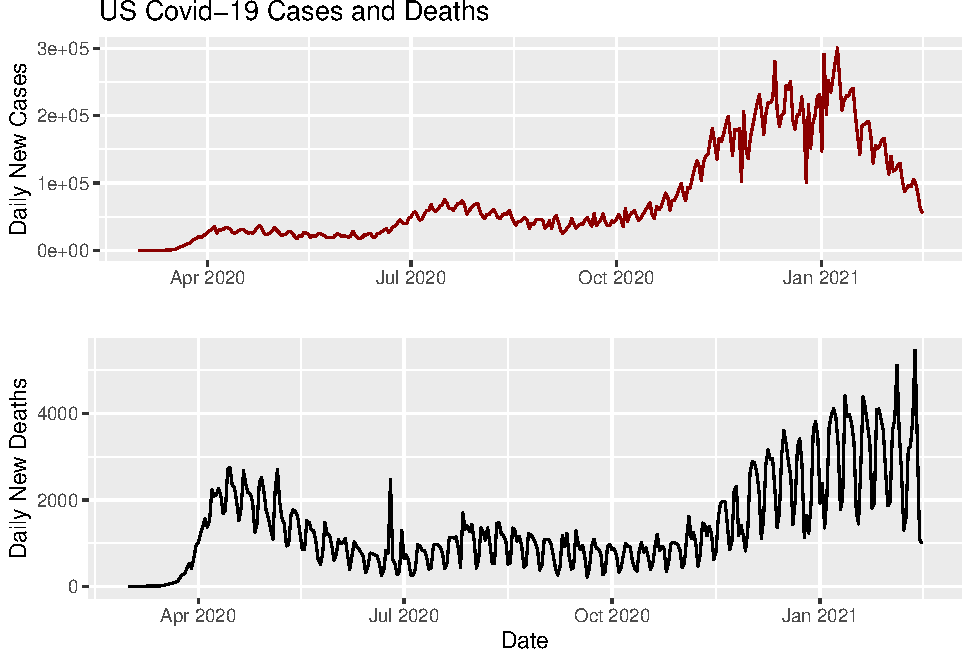
\includegraphics{figs/unnamed-chunk-2.pdf}

\begin{center}
Figure 1 - Timeseries of daily new Covid-19 cases (top) and deaths (bottom) in the United States, March 2020 - February 2021.
\end{center}

\hypertarget{case-death-scatter-plot}{%
\subsection{Case-Death Scatter Plot}\label{case-death-scatter-plot}}

To further examine how the relationship between daily new US covid cases
and deaths changed through time, a scatter plot of these two variables
was generated (Figure 2). Having previously identified four distinct
regimes in the case growth rate, these points were colored by the season
for each observation. The scatter plot further highlights the different
trends in the daily case to death ratios during each of these time
periods. In the spring 2020, there is an significantly evident positive
correlation in the case to death ratio. The points in this season are
all closely clustered with the deaths growing exponentially with cases.
In the summer 2020 data, there is no clear positive or negative trend in
the correlation between the two parameters with the points scatter
roughly in a circle. In the fall season, again a positive correlation is
evident, however the case to death ratio is four to five times that
observed in the spring. Finally in the winter (December 2020 -- February
2021), the ratio of cases to deaths decreases but is still positive.

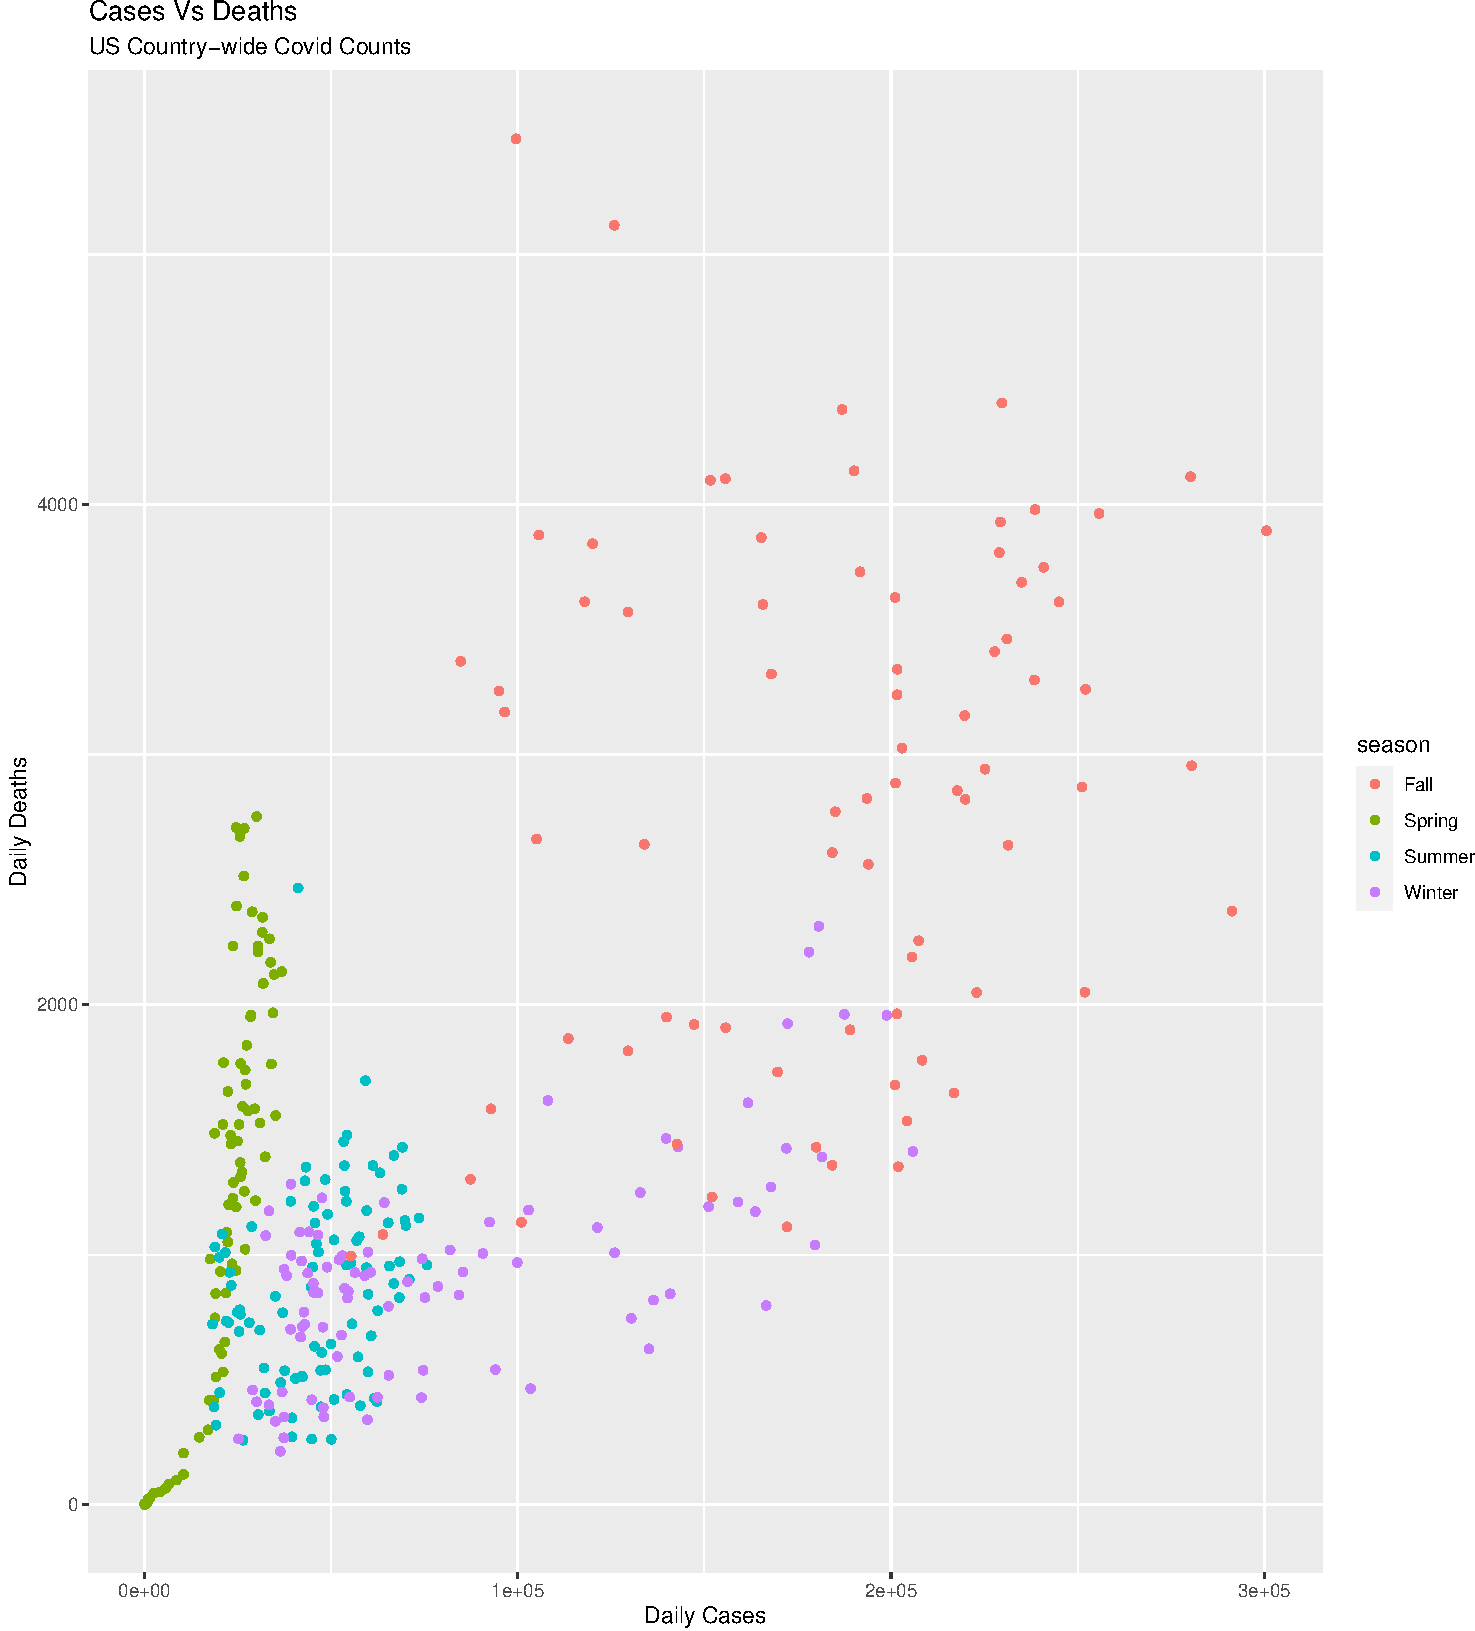
\includegraphics{figs/unnamed-chunk-3.pdf}

\begin{center}
Figure 2 - Scatterplot of daily new Covid-19 cases vs deaths in United States. Point colors indicate season
\end{center}

\hypertarget{state-case-rate-box-plots}{%
\subsection{State Case Rate Box Plots}\label{state-case-rate-box-plots}}

\begin{center}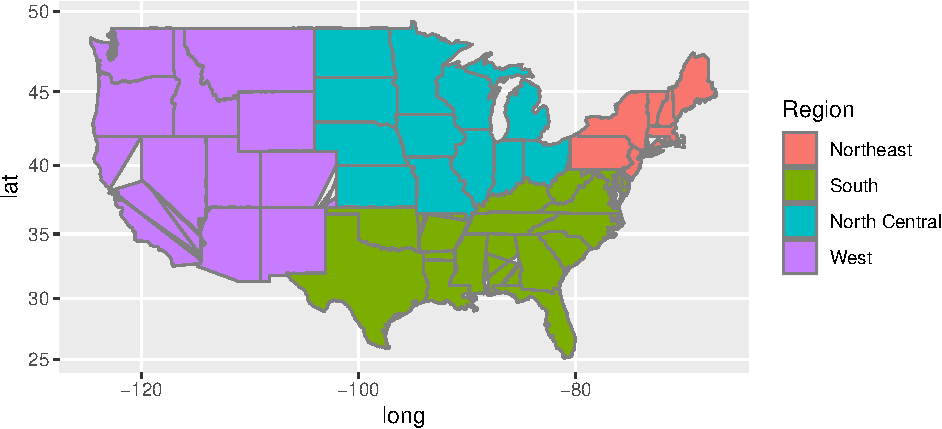
\includegraphics{figs/unnamed-chunk-4} \end{center}

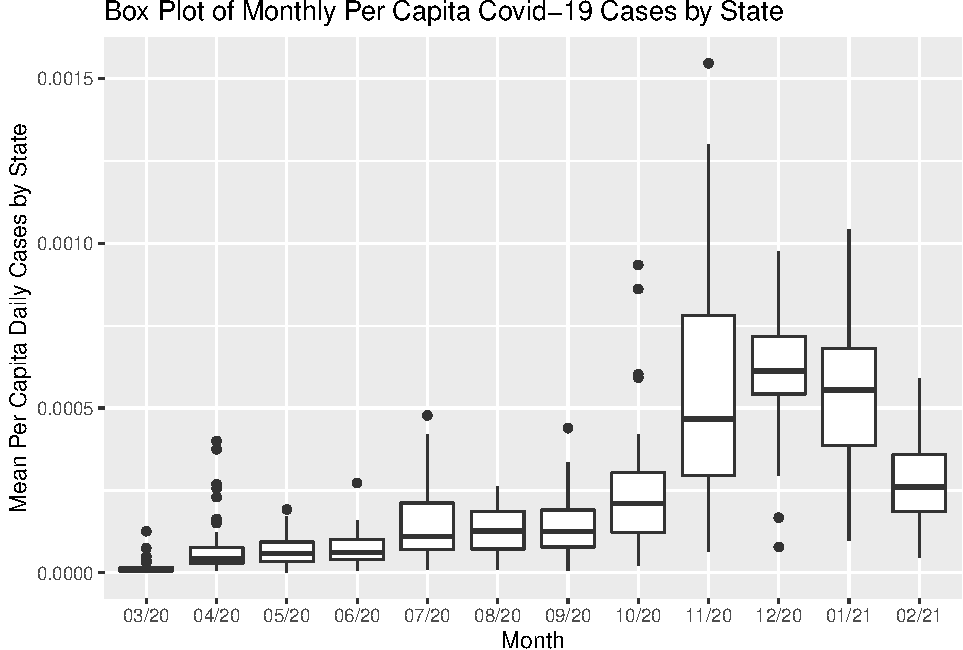
\includegraphics{figs/unnamed-chunk-5.pdf}

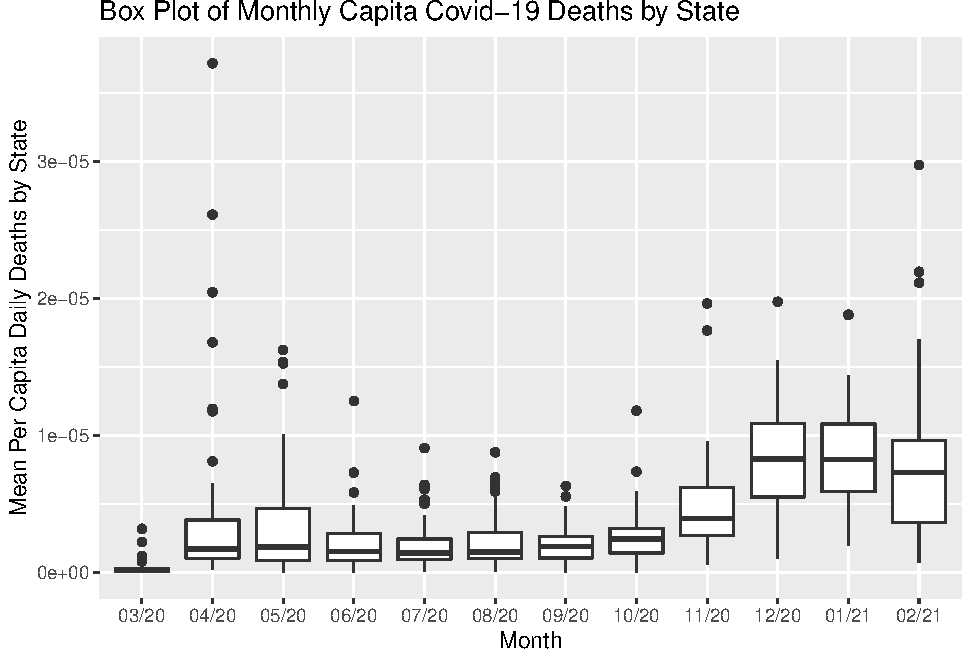
\includegraphics{figs/unnamed-chunk-6.pdf}

\begin{center}
Figure 3 - Map of US Regions
\end{center}

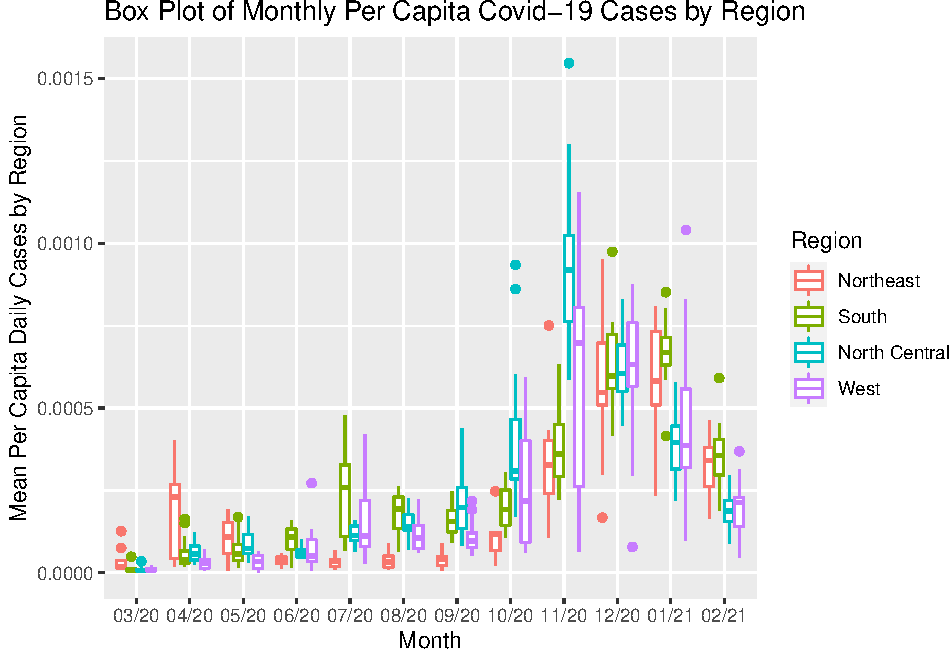
\includegraphics{figs/unnamed-chunk-7.pdf}

\begin{center}
Figure 4 - Boxplot
\end{center}

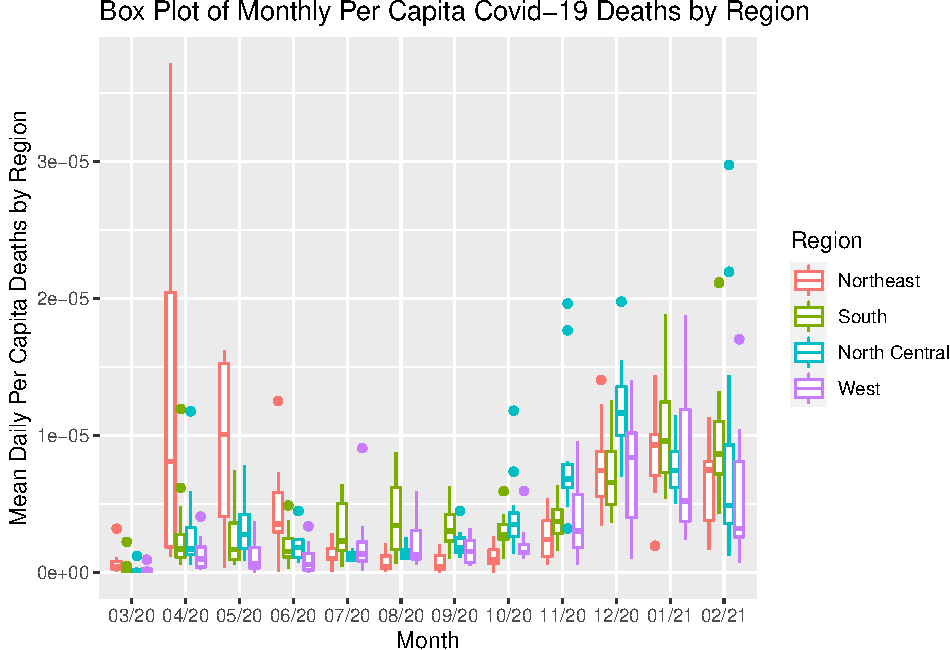
\includegraphics{figs/unnamed-chunk-8.pdf}

\textbackslash begin\{center\} Figure 4 - Boxplot
\textbackslash end\{center

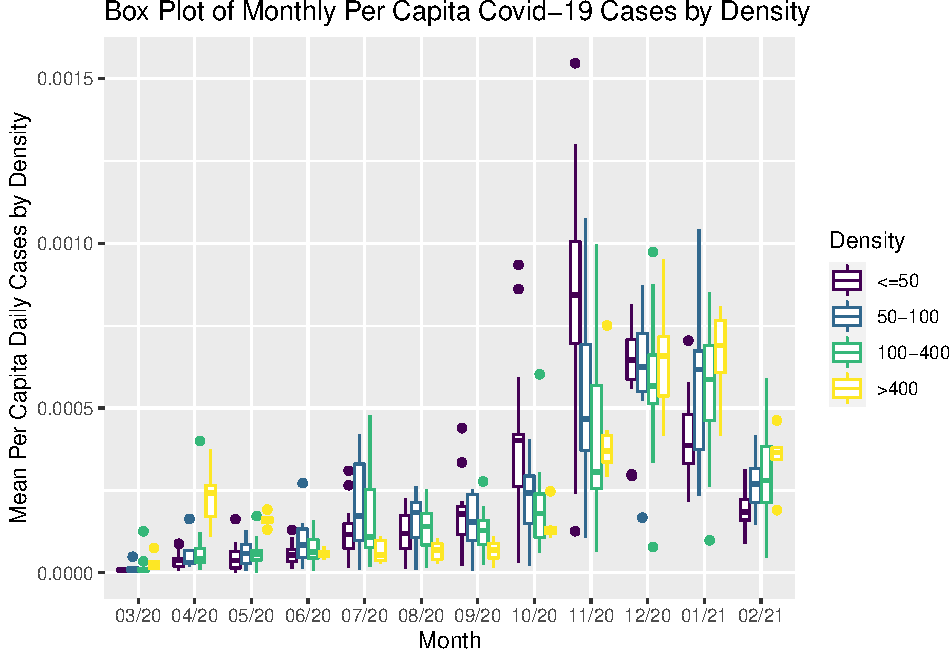
\includegraphics{figs/unnamed-chunk-9.pdf}

\textbackslash begin\{center\} Figure 4 - Boxplot
\textbackslash end\{center

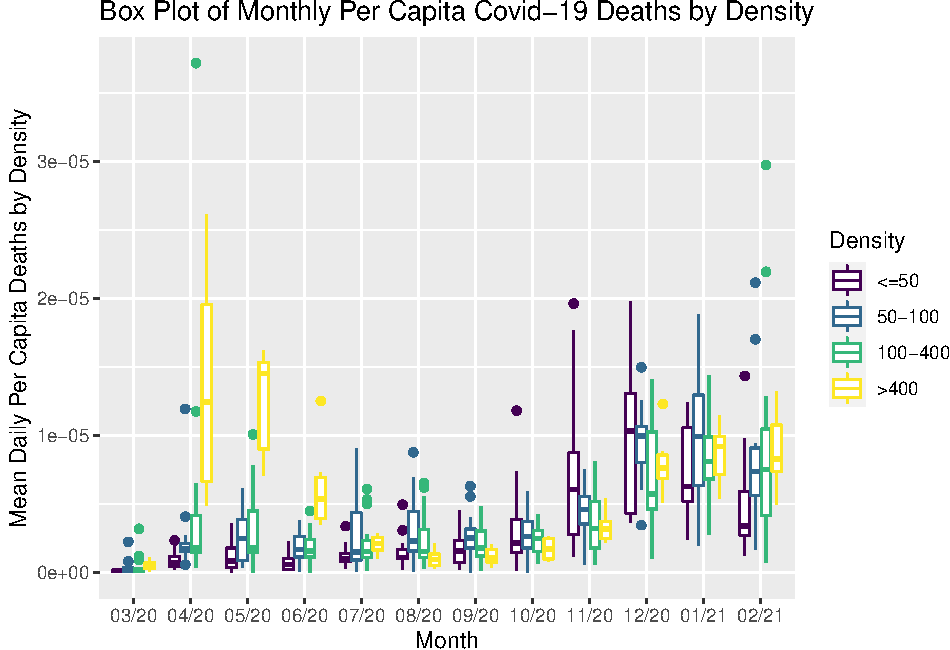
\includegraphics{figs/unnamed-chunk-10.pdf}

\textbackslash begin\{center\} Figure 4 - Boxplot
\textbackslash end\{center

\hypertarget{clustering-analysis}{%
\subsection{Clustering Analysis}\label{clustering-analysis}}

\hypertarget{results}{%
\section{Results}\label{results}}

\hypertarget{conclusions}{%
\section{Conclusions}\label{conclusions}}

\hypertarget{appendix}{%
\section{Appendix}\label{appendix}}





\newpage
\singlespacing 
\bibliography{master.bib}

\end{document}
